\documentclass[letterpaper]{sig-alternate}

\setlength{\paperheight}{11in}
\setlength{\paperwidth}{8.5in}
\usepackage[pass]{geometry}

\usepackage{graphicx}
\usepackage{filecontents}
\usepackage[hidelinks,draft]{hyperref}
\usepackage{cite}
\usepackage{enumitem}

\usepackage[hang]{footmisc}
\usepackage{microtype}
\usepackage{setspace}

\begin{filecontents*}{ESC.bib}

@misc{bbcsoundeffects,
  title={{BBC} Sound Effects Library},
  howpublished={\textls[-30]{\urlstyle{same}\url{http://www.sound-ideas.com/sound-effects/bbc-sound-effects.html}}},
  note={\textls[-30]{(\textit{Aug. 5, 2015})}}
}

@article{alexandre2007feature,
  title={Feature selection for sound classification in hearing aids through restricted search driven by genetic algorithms},
  author={Alexandre, E. and others},
  journal={IEEE Transactions on Audio, Speech, and Language Processing},
  volume={15},
  number={8},
  pages={2249--2256},
  year={2007},
  publisher={IEEE}
}

@inproceedings{ballan2009deep,
  title={Deep networks for audio event classification in soccer videos.},
  author={Ballan, L. and others},
  booktitle={Proceedings of the IEEE International Conference on Multimedia and Expo},
  pages={474--477},
  year={2009}
}

@article{barchiesi2015acoustic,
  title={Acoustic Scene Classification: Classifying environments from the sounds they produce},
  author={Barchiesi, D. and others},
  journal={Signal Processing Magazine},
  volume={32},
  number={3},
  pages={16--34},
  year={2015},
  publisher={IEEE}
}

@article{chachada2014environmental,
  title={Environmental sound recognition: A survey},
  author={Chachada, S. and Kuo, C.-C. J.},
  journal={APSIPA Transactions on Signal and Information Processing},
  volume={3},
  pages={e14},
  year={2014},
  publisher={Cambridge Univ Press}
}

@inproceedings{font2013freesound,
  title={Freesound technical demo},
  author={Font, F. and Roma, G. and Serra, X.},
  booktitle={Proceedings of the ACM International Conference on Multimedia},
  pages={411--412},
  year={2013},
  organization={ACM}
}

@inproceedings{giannoulis2013aasp,
  title={Detection and classification of acoustic scenes and events: {An IEEE AASP} challenge},
  author={Giannoulis, D. and others},
  booktitle={Proceedings of the IEEE Workshop on Applications of Signal Processing to Audio and Acoustics (WASPAA)},
  year={2013},
  organization={IEEE}
}

@inproceedings{lallemand2012content,
  title={Content-based Retrieval of Environmental Sounds by Multiresolution Analysis},
  author={Lallemand, I. and Schwarz, D. and Artieres, T.},
  booktitle={Proceedings of the Sound and Music Computing conference},
  year={2012}
}

@incollection{lopatka2010dangerous,
  title={Dangerous sound event recognition using support vector machine classifiers},
  author={{\L}opatka, K. and Zwan, P. and Czy{\.z}ewski, A.},
  booktitle={Advances in Multimedia and Network Information System Technologies},
  pages={49--57},
  year={2010},
  publisher={Springer}
}

@inproceedings{maxime2014sound,
  title={Sound representation and classification benchmark for domestic robots},
  author={Maxime, J. and others},
  booktitle={Proceedings of the IEEE International Conference on Robotics and Automation (ICRA)},
  pages={6285--6292},
  year={2014},
  organization={IEEE}
}

@inproceedings{nishiura2002evaluation,
  title={An evaluation of sound source identification with {RWCP} sound scene database in real acoustic environments},
  author={Nishiura, T. and Nakamura, S.},
  booktitle={Proceedings of the IEEE International Conference on Multimedia and Expo},
  volume={2},
  pages={265--268},
  year={2002},
  organization={IEEE}
}

@inproceedings{piczak2015esc-convnet,
  title={Environmental Sound Classification with Convolutional Neural Networks},
  author={Piczak, K. J.},
  booktitle={Proceedings of the IEEE International Workshop on Machine Learning for Signal Processing (MLSP)},
  year={2015},
  organization={IEEE},
  note={\textit{In press}}  
}

@inproceedings{plinge2014bag,
  title={A bag-of-features approach to acoustic event detection},
  author={Plinge, A. and others},
  booktitle={Proceedings of the IEEE International Conference on Acoustics, Speech and Signal Processing (ICASSP)},
  pages={3704--3708},
  year={2014},
  organization={IEEE}
}

@inproceedings{salamon2014dataset,
  title={A dataset and taxonomy for urban sound research},
  author={Salamon, J. and Jacoby, C. and Bello, J. P.},
  booktitle={Proceedings of the ACM International Conference on Multimedia},
  pages={1041--1044},
  year={2014},
  organization={ACM}
}

@article{stowell2013open,
  title={An open dataset for research on audio field recording archives: freefield1010},
  author={Stowell, D. and Plumbley, M. D.},
  journal={arXiv preprint arXiv:1309.5275},
  year={2013}
}


@inproceedings{vacher2007sound,
  title={Sound classification in a smart room environment: an approach using {GMM} and {HMM} methods},
  author={Vacher, M. and Serignat, J.-F. and Chaillol, S.},
  booktitle={Proceedings of the IEEE Conference on Speech Technology and Human-Computer Dialogue},
  pages={135--146},
  year={2007}
}

@inproceedings{van2009dares,
  title={{DARES-G1: Database} of annotated real-world everyday sounds},
  author={van Grootel, M. and Andringa, T. and Krijnders, J.},
  booktitle={Proceedings of the NAG/DAGA International Conference on Acoustics},
  year={2009}
}

\end{filecontents*}


\newfont{\mycrnotice}{ptmr8t at 7pt}
\newfont{\myconfname}{ptmri8t at 7pt}
\let\crnotice\mycrnotice%
\let\confname\myconfname%

\permission{Permission to make digital or hard copies of all or part of this work for personal or classroom use is granted without fee provided that copies are not made or distributed for profit or commercial advantage and that copies bear this notice and the full citation on the first page. Copyrights for components of this work owned by others than the author(s) must be honored. Abstracting with credit is permitted. To copy otherwise, or republish, to post on servers or to redistribute to lists, requires prior specific permission and/or a fee. Request permissions from Permissions@acm.org.}
\conferenceinfo{MM'15,}{October 26--30, 2015, Brisbane, Australia. \\ 
{\mycrnotice{Copyright is held by the owner/author(s). Publication rights licensed to ACM.}}}
\copyrightetc{ACM \the\acmcopyr}
\crdata{978-1-4503-3459-4/15/10\ ...\$15.00.\\
DOI: http://dx.doi.org/10.1145/2733373.2806390}

\clubpenalty=10000 
\widowpenalty=10000

\lefthyphenmin=3
\hyphenation{analy-sis}

\begin{document}

\renewcommand{\footnotesize}{\fontsize{7pt}{9pt}\selectfont}
\setlength\footnotemargin{8pt}

\title{ESC: Dataset for Environmental Sound Classification}

\numberofauthors{1}
\author{
\alignauthor
Karol J. Piczak\\
       \affaddr{Institute of Electronic Systems}\\
       \affaddr{Warsaw University of Technology}\\
       \affaddr{Warsaw, Poland}\\
       \email{K.Piczak@stud.elka.pw.edu.pl}
}

\maketitle
\begin{abstract}
One of the obstacles in research activities concentrating on environmental sound classification is the scarcity of suitable and publicly available datasets. This paper tries to address that issue by presenting a new annotated collection of 2~000 short clips comprising 50 classes of various common sound events, and an abundant unified compilation of 250~000 unlabeled auditory excerpts extracted from recordings available through the Freesound project. The paper also provides an evaluation of human accuracy in classifying environmental sounds and compares it to the performance of selected baseline classifiers using features derived from mel-frequency cepstral coefficients and zero-crossing rate.
\end{abstract}

\category{H.3.1}{Information Systems}{Content Analysis and Indexing}
\category{H.5.5}{Information Systems}{Sound and Music Computing}

\keywords{environmental sound; classification; dataset}

\section{Introduction}
Recent years have brought a steady stream of advances in machine perception. Computer systems undertake progressively more complex tasks, at times even surpassing human capabilities. A significant part of these spectacular achievements has come in visual recognition, with recent proliferation of successful deep learning approaches.

At the same time, research in auditory recognition tasks has been focusing mostly on speech and music processing. Analysis of environmental sounds (a very diverse group of everyday audio events which cannot be described as speech nor music) has lagged behind in applying those recent improvements, despite numerous possible applications in audio surveillance systems~\cite{lopatka2010dangerous}, hearing aids~\cite{alexandre2007feature}, smart room monitoring~\cite{vacher2007sound}, and video content highlight generation~\cite{ballan2009deep}.

One of the objective impediments to more active research in this field is strong fragmentation and difficulty in comparability and reproducibility. Most studies so far (Barchiesi et~al.~\cite{barchiesi2015acoustic} and Chachada \& Kuo~\cite{chachada2014environmental} present recent surveys of this topic) have been conducted on datasets that are either very specific, small, or (semi-)proprietary~\cite{giannoulis2013aasp, bbcsoundeffects, maxime2014sound, stowell2013open, lallemand2012content, nishiura2002evaluation, van2009dares, plinge2014bag}. This scarcity of publicly available datasets\footnote{Most datasets are listed on a website maintained by Toni Heittola:\newline\textls[-25]{\urlstyle{same}\url{http://www.cs.tut.fi/~heittolt/datasets.html} [\textit{Accessed Aug. 5, 2015}]}} and difficulty in accessing the original code for study replication make research reproducibility efforts harder than they should be. That is in stark contrast to such fields as computer vision where corpora like MNIST\footnote{\urlstyle{same}\textls[-25]{\url{http://yann.lecun.com/exdb/mnist/} [\textit{Accessed Aug. 5, 2015}]}} and CIFAR\footnote{\urlstyle{same}\textls[-25]{\url{http://www.cs.toronto.edu/~kriz/cifar.html} [\textit{Accessed Aug. 5, 2015}]}} have been prominently used as a~de~facto standard for baseline comparisons. Only in the recent months did initiatives such as the Urban Sound project~\cite{salamon2014dataset} (a dataset of recordings concentrating on urban environments) bring some hope for a change in this matter. The situation, however, still remains rather bleak.

Therefore, the goal of this paper is to facilitate open research in the field of environmental sound classification by:

\begin{itemize}[noitemsep,topsep=0pt]
\item contributing a publicly available dataset of environmental recordings,
\item presenting estimates of human classification accuracy for this dataset,
\item comparing these numbers with baseline performance of most common machine learning classifiers,
\item providing a Jupyter (IPython) notebook with a more thorough analysis and code for easy replication of obtained results.
\end{itemize}

\section{The ESC dataset}

The presented compilation consists of three parts: the main labeled set comprising 50 classes of various environmental sounds, a small proof-of-concept subset of 10 classes selected from the main dataset - serving as a simplified benchmark - and a supplementary dataset of unlabeled excerpts suitable for unsupervised learning experiments.

All datasets consist of sound clips constructed from recordings available publicly through the Freesound project~\cite{font2013freesound}. Classes included in the labeled part of the dataset were arbitrarily selected with the goal of maintaining balance between major types of sound events, all the while taking into consideration the limitations in the number and diversity of available source recordings, and subjectively assessed usefulness and distinctiveness of each class. The Freesound database of field recordings was queried for common terms related to the constructed classes. Search results were individually evaluated and verified by the author by annotating fragments containing events belonging to the given class. These annotations were then used to extract 5-second-long recordings of audio events (shorter events were padded with silence as needed). The extracted samples were reconverted to a unified format (44.1~kHz, single channel, Ogg Vorbis compression at 192~kbit/s). The labeled datasets were consequently arranged into 5 uniformly sized cross-validation folds, ensuring that clips originating from the same initial source file are always contained in a single fold.

The resulting dataset is available under a Creative Commons non-commercial license through the Harvard Dataverse project\footnote{\urlstyle{same}\textls[-25]{\url{http://dx.doi.org/10.7910/DVN/YDEPUT}}}. It is accompanied by an IPython notebook containing a more thorough analysis of the dataset than is possible in a short paper format, and the detailed results obtained along with source code for study replication\footnote{
\urlstyle{same}\textls[-25]{\url{https://github.com/karoldvl/paper-2015-esc-dataset}}

}.  

\subsection{ESC-50}

The \textit{ESC-50} dataset consists of 2~000 labeled environmental recordings equally balanced between 50 classes (40 clips per class). For convenience, they are grouped in 5 loosely defined major categories (10 classes per category):

\begin{itemize}[noitemsep,topsep=0pt]
\itemsep0em
\item animal sounds,
\item natural soundscapes and water sounds,
\item human (non-speech) sounds,
\item interior/domestic sounds,
\item exterior/urban noises.
\end{itemize}

The goal of the extraction process was to keep sound events exposed in the foreground with limited background noise when possible. However, field recordings are far from sterile, thus some clips may still exhibit auditory overlap in the background.

The dataset provides an exposure to a variety of sound sources - some very common (\textit{laughter}, \textit{cat meowing}, \textit{dog barking}), some quite distinct (\textit{glass breaking}, \textit{brushing teeth}) and then some where the differences are more nuanced (\textit{helicopter} and \textit{airplane} noise).

One of the possible deficiencies of this dataset is the limited number of clips available per class. This is related to the high cost of manual annotation and extraction, and the decision to maintain strict balance between classes despite limited availability of recordings for more exotic types of sound events. Nevertheless, it will, hopefully, be useful in its current form and is a concept that could be expanded on if sufficient interest is expressed.

\subsection{ESC-10}

The \textit{ESC-10} is a selection of 10 classes from the bigger dataset, representing three general groups of sounds:

\begin{itemize}[noitemsep,topsep=0pt]
\item transient/percussive sounds, sometimes with very meaningful temporal patterns (\textit{sneezing}, \textit{dog barking}, \textit{clock ticking}),
\item sound events with strong harmonic content (\textit{crying baby}, \textit{crowing rooster}),
\item more or less structured noise/soundscapes (\textit{rain}, \textit{sea waves}, \textit{fire crackling}, \textit{helicopter}, \textit{chainsaw}).
\end{itemize}

This subset should provide an easier problem to start with, and it was initially constructed as a proof-of-concept dataset. The task of classifying sounds from such a constrained set of classes, a trivial feat from a human perspective, sets the bar really high for accuracy expected from automatic sound recognition systems. Therefore, this subset presents a~slightly different problem to tackle than the whole \textit{ESC-50} dataset. The differences between classes are much more pronounced, with limited ambiguity, and as such it may favor a different kind of machine learning approaches.

\subsection{ESC-US}

Unfortunately, the limited number of instances available in the labeled part of the dataset makes it rather inadequate for more complex knowledge discovery approaches like learning representations from data. To mitigate this issue, an additional dataset of 250 000 recordings (extracted from Freesound files tagged as ``field recording") is provided in the same short-clip (5-second-long) format. It should be more fitting for procedures involving unsupervised pre-training and generative models.

Although the \textit{ESC-US} dataset should be treated as not hand-annotated and is presented as such, it does include the metadata (tags/sound descriptions) submitted for the original recordings. However, in contrast to the labeled part of the dataset, the metadata were not verified individually by the author, but rely solely on Freesound's quality control procedures through crowd moderation.

Therefore, the dataset, apart from clustering and manifold learning experiments, could be also used in weakly supervised learning regimes (classification with labels partially missing or not specific enough).

\section{Sound classification}

\subsection{Human classification accuracy}

The human auditory system has little problem recognizing a plethora of sound stimuli, even in very noisy conditions. Therefore, it is to be expected that, with such a limited challenge as presented by the dataset, proper recognition of sound events should not be difficult at all. The real question was: how easy is it? To answer this, numerous participants were asked through the CrowdFlower crowdsourcing platform to try their best at classifying sounds from the labeled datasets.

The experiment involved presenting a number of sound recordings to participants and asking them to choose a correct label from a list of 10 or, respectively, 50 categories. The participants were paid a flat fee per unit of work (classifying 10 recordings). Quality control was maintained through internal CrowdFlower's procedures (participant pre-screening and ongoing monitoring through randomly inserted test questions with an expected answer). The final results were further assessed by the author for potential outliers, and a small number of entries were eliminated this way. In total around 4~000 judgments were collected for each dataset (on average a dozen human classification entries per individual clip of \textit{ESC-10} and two for \textit{ESC-50}). Although it is hard to come up with formal statistical interpretation with such an experiment setup, it should nevertheless provide a rough estimate of human capabilities in recognizing everyday sounds.

The average accuracy achieved was 95.7\% for the \textit{ESC-10} dataset and 81.3\% for \textit{ESC-50}. Recall for individual classes varied greatly between types of sound events - from 34.1\% for washing machine noise to almost 100\% for crying babies and barking dogs. Without going too much into details\footnote{Full experiment results are available as a spreadsheet supplementing the dataset, and a more thorough analysis is performed as part of the provided IPython notebook.}, sound events presented in the dataset can be divided into three groups based on their difficulty level:

\begin{itemize}[noitemsep,topsep=0pt]
\itemsep0em
\item easy categories (most human sounds, animals, and some very distinct sound sources, like \textit{siren}, \textit{water drops}, \textit{breaking glass}),
\item average categories (everything in between the other two),
\item difficult categories (mostly soundscapes and various mechanical noises).
\end{itemize}

One of the problems in such experiments is that with increasing number of categories, it becomes more difficult for untrained participants to mentally grasp all the possibilities and semantic differences. With 50 classes of sound events, it was still possible to provide them in one coherent view (divided into 5 major groups for faster orientation) without reaching for nested taxonomies, but it was on the verge of what is verifiable in such an experiment setup.

Nevertheless, based on these experiments, one can expect that trained and attentive listeners could score flawlessly on the smaller dataset and most probably achieve accuracy levels reaching 90\% on the main dataset, with some room for error when classifying more ambiguous mechanical noises and soundscapes.

\renewcommand{\topfraction}{0.8}
\renewcommand{\floatpagefraction}{0.8}

\begin{figure}
\centering
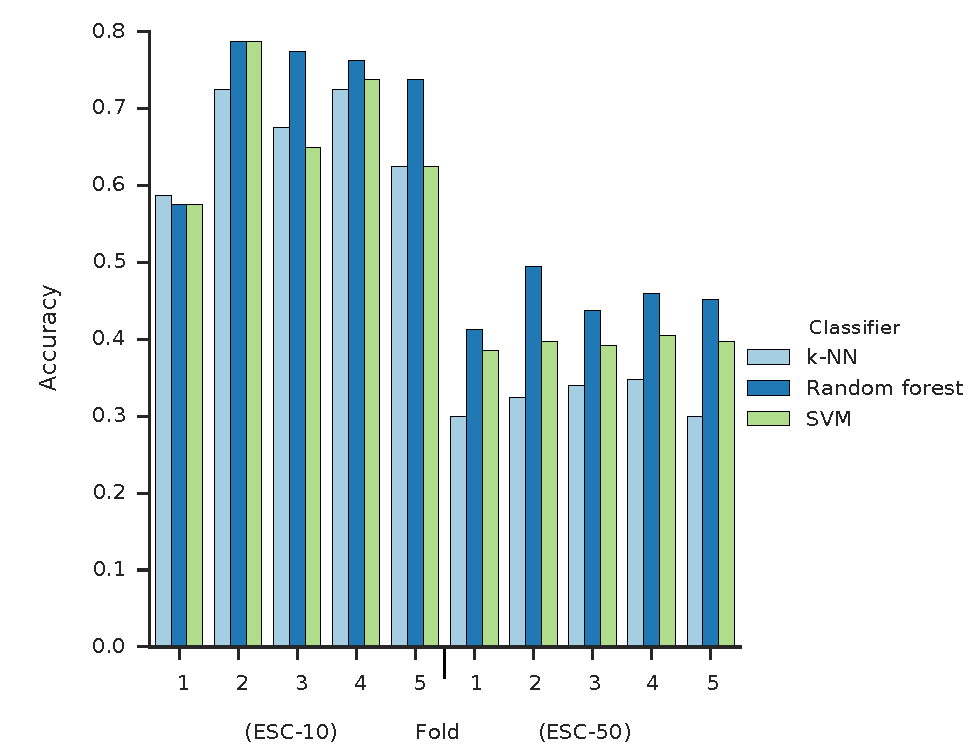
\includegraphics[width=20pc]{Figures/figure_accuracy_folds.pdf}
\caption{\label{fig:accuracy}Comparison of classification accuracy between folds depending on the choice of classifier.}
\vspace{-12pt}
\end{figure}

\begin{figure}
\centering
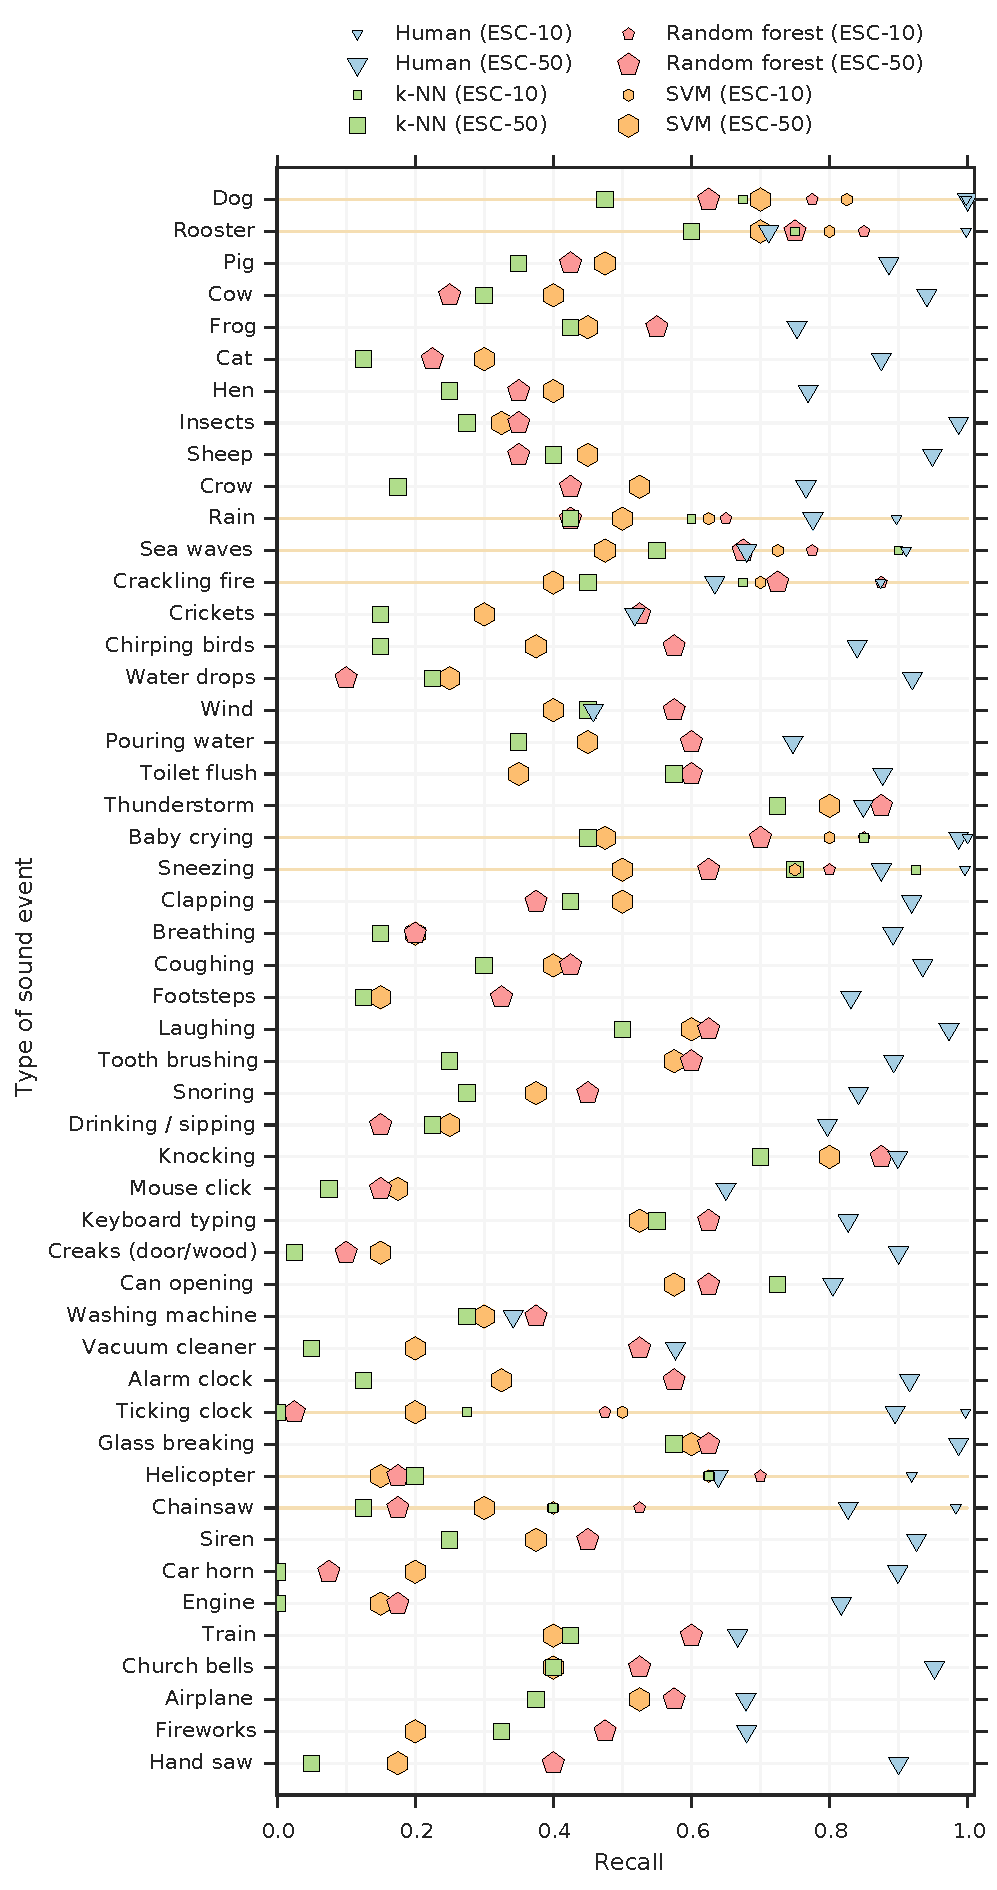
\includegraphics[width=20pc]{Figures/figure_recall.pdf}
\caption{\label{fig:recall}Category recall for different types of classifiers and human assessment.}
\vspace{-12pt}
\end{figure}

\subsection{Baseline machine classification results}

Having established an approximate figure on what is the desired target accuracy for a sound recognition system with near-human capacity, the second goal was to verify what can be achieved with some baseline approaches to machine classification of environmental sounds. The aim of this analysis was not to construct the most robust system possible, but to investigate what can be done with basic approaches, exploring potential pitfalls and intricacies of the dataset.

Two types of features were extracted from each clip: zero-crossing rate and mel-frequency cepstral coefficients (\textit{MFCC}). The former is a very simple, yet useful feature, whereas the latter are ubiquitous in speech processing and analyzing harmonic content. MFCCs were computed using the librosa package\footnote{\textit{librosa: v0.3.1} library by B. McFee et al.,\newline \textls[-30]{DOI: \urlstyle{same}\url{http://dx.doi.org/10.5281/zenodo.12714} [\textit{Accessed Aug. 5, 2015}]}} with default settings resulting in frame length of 11.6~ms. Discarding the 0th~coefficient, first 12~MFCCs and zero-crossing rate were summarized for each clip with their mean and standard deviation across frames. Feature vectors created in this way were treated as input to three types of classifiers: k-nearest neighbors (\textit{k-NN}), random forest ensemble and support vector machine (\textit{SVM}) with linear kernel. Learning was performed on both datasets with a~5-fold cross-validation regime.

The \textit{ESC-10} dataset had an average classification accuracy ranging from 66.7\% for the k-NN classifier to 72.7\% for the random forest ensemble, with SVM in the middle (67.5\%). Some significant dispersion in results achieved could be seen between folds, owing to their small absolute size (see figure~\ref{fig:accuracy}). The \textit{ESC-50} dataset had less variability between folds when validating the models, but more pronounced outperformance by the random forest ensemble (44.3\%) as compared to SVM (39.6\%) or k-NN (32.2\%).

One tendency that stands out when contrasting performance of different classifiers on both datasets is the pronounced drop in accuracy for the simplest (k-NN) model. It could indicate that the dependencies between features were more intricate in the bigger dataset, and they were better captured with more complex models.

In general, these rudimentary classification systems performed poorly when contrasted with their human counterparts, yet the difference is more pronounced for some groups of sounds than the others (see figure~\ref{fig:recall}). For instance, lots of recordings in soundscape/background noise categories prove to be quite ambiguous for human listeners, a group which coincidentally scores quite high with automated systems.

The SVM classifier performed better for animal sounds than the random forest ensemble. Although a possible artifact of the data, it may also indicate that using more customized models for specific broader groups of sounds could be a viable option (creating a form of hierarchical multi-stage classification system).

It should be noted that the presented baseline classification methods are relatively simple. An evaluation of more robust approaches (based on convolutional neural networks) is performed in a more recent work of the author~\cite{piczak2015esc-convnet}.

\vspace{-2pt}

\section{Summary}

The aim of this paper was to present a new compilation of environmental recordings that could enrich the research domain not so abundant with publicly available datasets. Hopefully, this material will help foster more open research efforts in analyzing environmental sounds.

There are numerous possible ways to expand on this topic, some of which include:

\begin{itemize}[noitemsep,topsep=0pt]
\item compiling a fully replicable survey comparing various approaches utilized in past research papers,
\item evaluating deep neural networks and other deep learning models in the context of environmental sound classification, e.g. with unsupervised pre-training using the \textit{ESC-US} dataset,
\item exploring the \textit{ESC-US} dataset and the research possibilities it creates (clustering techniques, using available metadata in weakly-supervised setting or a hybrid machine-crowd annotation project, manifold learning etc.).
\end{itemize}

\vspace{-8pt}

\section*{Acknowledgments}

I would like to thank Frederic Font for his help in using the Freesound API and anonymous reviewers for their thorough and helpful comments.

\bibliographystyle{abbrv}
\bibliography{ESC}

%\balancecolumns

\end{document}